% !TeX program=lualatex 
% !TeX spellcheck = de_DE
% !TeX encoding = utf8
% !TeX TXS-program:bibliography = txs:///biber
%%magic comment: einige Editoren verstehen diese Kommentare und starten lualatex anstatt der Standardeinstellung als Compiler



\showboxdepth=\maxdimen
\showboxbreadth=\maxdimen



\documentclass[ngerman]{mucproc}


%%%%%%%%%%%%%%%%%
%Quellen
\usepackage{pdfpages}

\addbibresource{DLN.bib}
\providecommand{\apashortdash}{-}
\usepackage[T1]{fontenc}       %% Schriftkodierung, die nativ Umlaute unterstützt
\usepackage[utf8]{inputenc}  %% Umlaute direkt eingeben
\usepackage{mathptmx}          %% schmal laufende Times als Brotschrift
\usepackage[scaled=.92]{helvet}%% Helvetica als Grotesk
% \usepackage[scaled=.87]{luximono} %% anderer Monotype-Font
\usepackage{geometry}          %% damit auch das Papierformat passt

\usepackage{booktabs}          %% schönere Tabellenlinien
\usepackage{graphicx}          %% Graphiken einbinden


\usepackage{csquotes} %% autom. Anführungszeichen
%% Literaturverzeichnisse: Hier ist nichts spezielles. Wählen Sie, was
%% Sie aus babelbib brauchen.
\usepackage[%
backend=biber,              %% Biber verwenden.
]{biblatex} 





%%%%%%%%%%%%%%%%%
%Für Tabellenbeispiel
\usepackage{tabularx}
\usepackage{booktabs}
%%%%%%%%%%%%%%%%%


\usepackage{subfig,graphicx}

%%%%%%%%%%%%%%%%%
%Nur wegen der Codebeispiele notwendig

%%%SyntaxHighlighting: Needs pygmentize installed and -shell-escape set. See minted-documentation for for information.
%\usepackage{minted}
%\setminted{bgcolor=black!10,tabsize=4}
%\NewDocumentCommand{\inlinemint}{O{}mv}{\mintinline[#1]{#2}{#3}}
%\usemintedstyle{friendly}

\usepackage{listings}

%%Fallback wenn minted nicht konfiguriert ist
\usepackage{verbatim}% http://ctan.org/pkg/verbatim
\newenvironment{minted}[2][]{\endgraf\verbatim}{\endverbatim}
\NewDocumentCommand{\inlinemint}{omv}{\texttt{#3}}


%Symbol-Font: Sonst sind die Symbolschriftarten nicht voll skalierbar
%\usepackage{unicode-math}
%\setmathfont{Latin Modern Math}
%%%%%%%%%%%%%%%%


%%%%%%%%%%%%%%%%%%%%%%%%%%%%%%%%%%%%%%%%%%%%%%%%%%%%%%%%%%%%%%%%%%%%%%%%%%%%%%%%%%%%%%%%%%%%%%%%%%%%%%%%%%%%%%%%%%%%%%%%%%%%%%%%%%%%%%%%%%%%
\begin{document}
	\title{MPPT-Laderegler Monitoring über einen Web Server mit dem ESP32 }
	\author{Harun Dastekin s0551006\thanks[HTW Berlin]{Studiengang: Angewandte Informatik, Drahtlose Netzwerke}}
	\email{Harun.Dastekin@Student.HTW-Berlin.de}
	
\maketitle
%%%%%%%%%%%%%%%%%%%%%%%%%%%%%%%%%%%%%%%%%%%%%%%%%%%%%%%%%%%%%%%%%%%%%%

%%%%%%%%%%%%%%%%%%%%%%%%%%%%%%%%%%%%%%%%%%%%%%%%%%%%%%%%%%%%%%%%%%%%%	
\begin{abstract}
Dieser Projektbericht behandelt ein Monitoring System für eine kleine Solaranlage mit Batteriespeicher. Ein ESP32 Node MCU misst anhand von Sensoren den Strom und die Spannung des Solarmoduls und überträgt diese an einen grafisch aufbereiteten Web Server. 
\end{abstract}	
%%%%%%%%%%%%%%%%%%%%%%%%%%%%%%%%%%%%%%%%%%%%%%%%%%%%%%%%%%%%%%%%%%%%%%%%%%%%%%%%%%%%%%%%%%%%%%%%%%%%%%%%%%%%%%%%%%%%%%%%%%%%%%%%%%%%%%%%%%%%
	
\section{Einleitung}
	In unserer heutigen Zeit ist ein Zugang zu Stromanschlüssen maßgeblich entscheidend für den Komfort. Oft liegt aber eine Steckdose nich genau dort wo man sie gerne hätte. Abhilfe sorgen dafür Solaranlagen die im besten Fall im Inselbetrieb arbeiten können. Mit anderen worten ein abgeschlossenes Energiesystem mit Energiezufuhr, Energiespeicher und einer möglichkeit diese Energie zu nutzen. Um den Energiegewinn ideal zu gestalten gibt es mehrere Faktoren die das beeinflussen. Darunter auch das Zusammenspiel zwischen der Energiezufuhr und dem Energiespeicher mit dem Verbrauch. D.h. eine Solarbatterie darf weder überladen noch tiefenentladen werden. Es muss eine Ladekurve geben, die den Ladevorgang reguliert. Um das zu bewerkstelligen benötigt es ein überwachungssystem der fließenden Ströme und der anliegenden Spannungen. Dazu wäre ein erster Schritt diese Anlage überwachen zu können und darauf geht diese Projektarbeit ein. Ein ähnliches Projekt habe ich im nachhinein auf dieser Internetseite gefunden\parencite{Monitoring.2021}.

%%%%%%%%%%%%%%%%%%%%%%%%%%%%%%%%%%%%%%%%%%%%%%%%%%%%%%%%%%%%%%%%%%%%%%%%%%%%%%%%%%%%%%%%%%%%%%%%%%%%%%%%%%%%%%%%%%%%%%%%%%%%%%%%%%%%%%%%%%%%
\newpage
\section{Haupteil}

	\subsection{Bauteile}
		

	Die Solaranlage besteht im Grunde genommen aus drei bzw. vier Bestandteilen. Einer 12V Batterie \ref{fig:Batterie}, einem Laderegler \ref{fig:Laderegler} und dem Photovoltaikmodul \ref{fig:Solarmodul} und gegebenenfalls einem Verbraucher.

\begin{figure}\centering
\subfloat[12V-Batterie]{\label{fig:Batterie}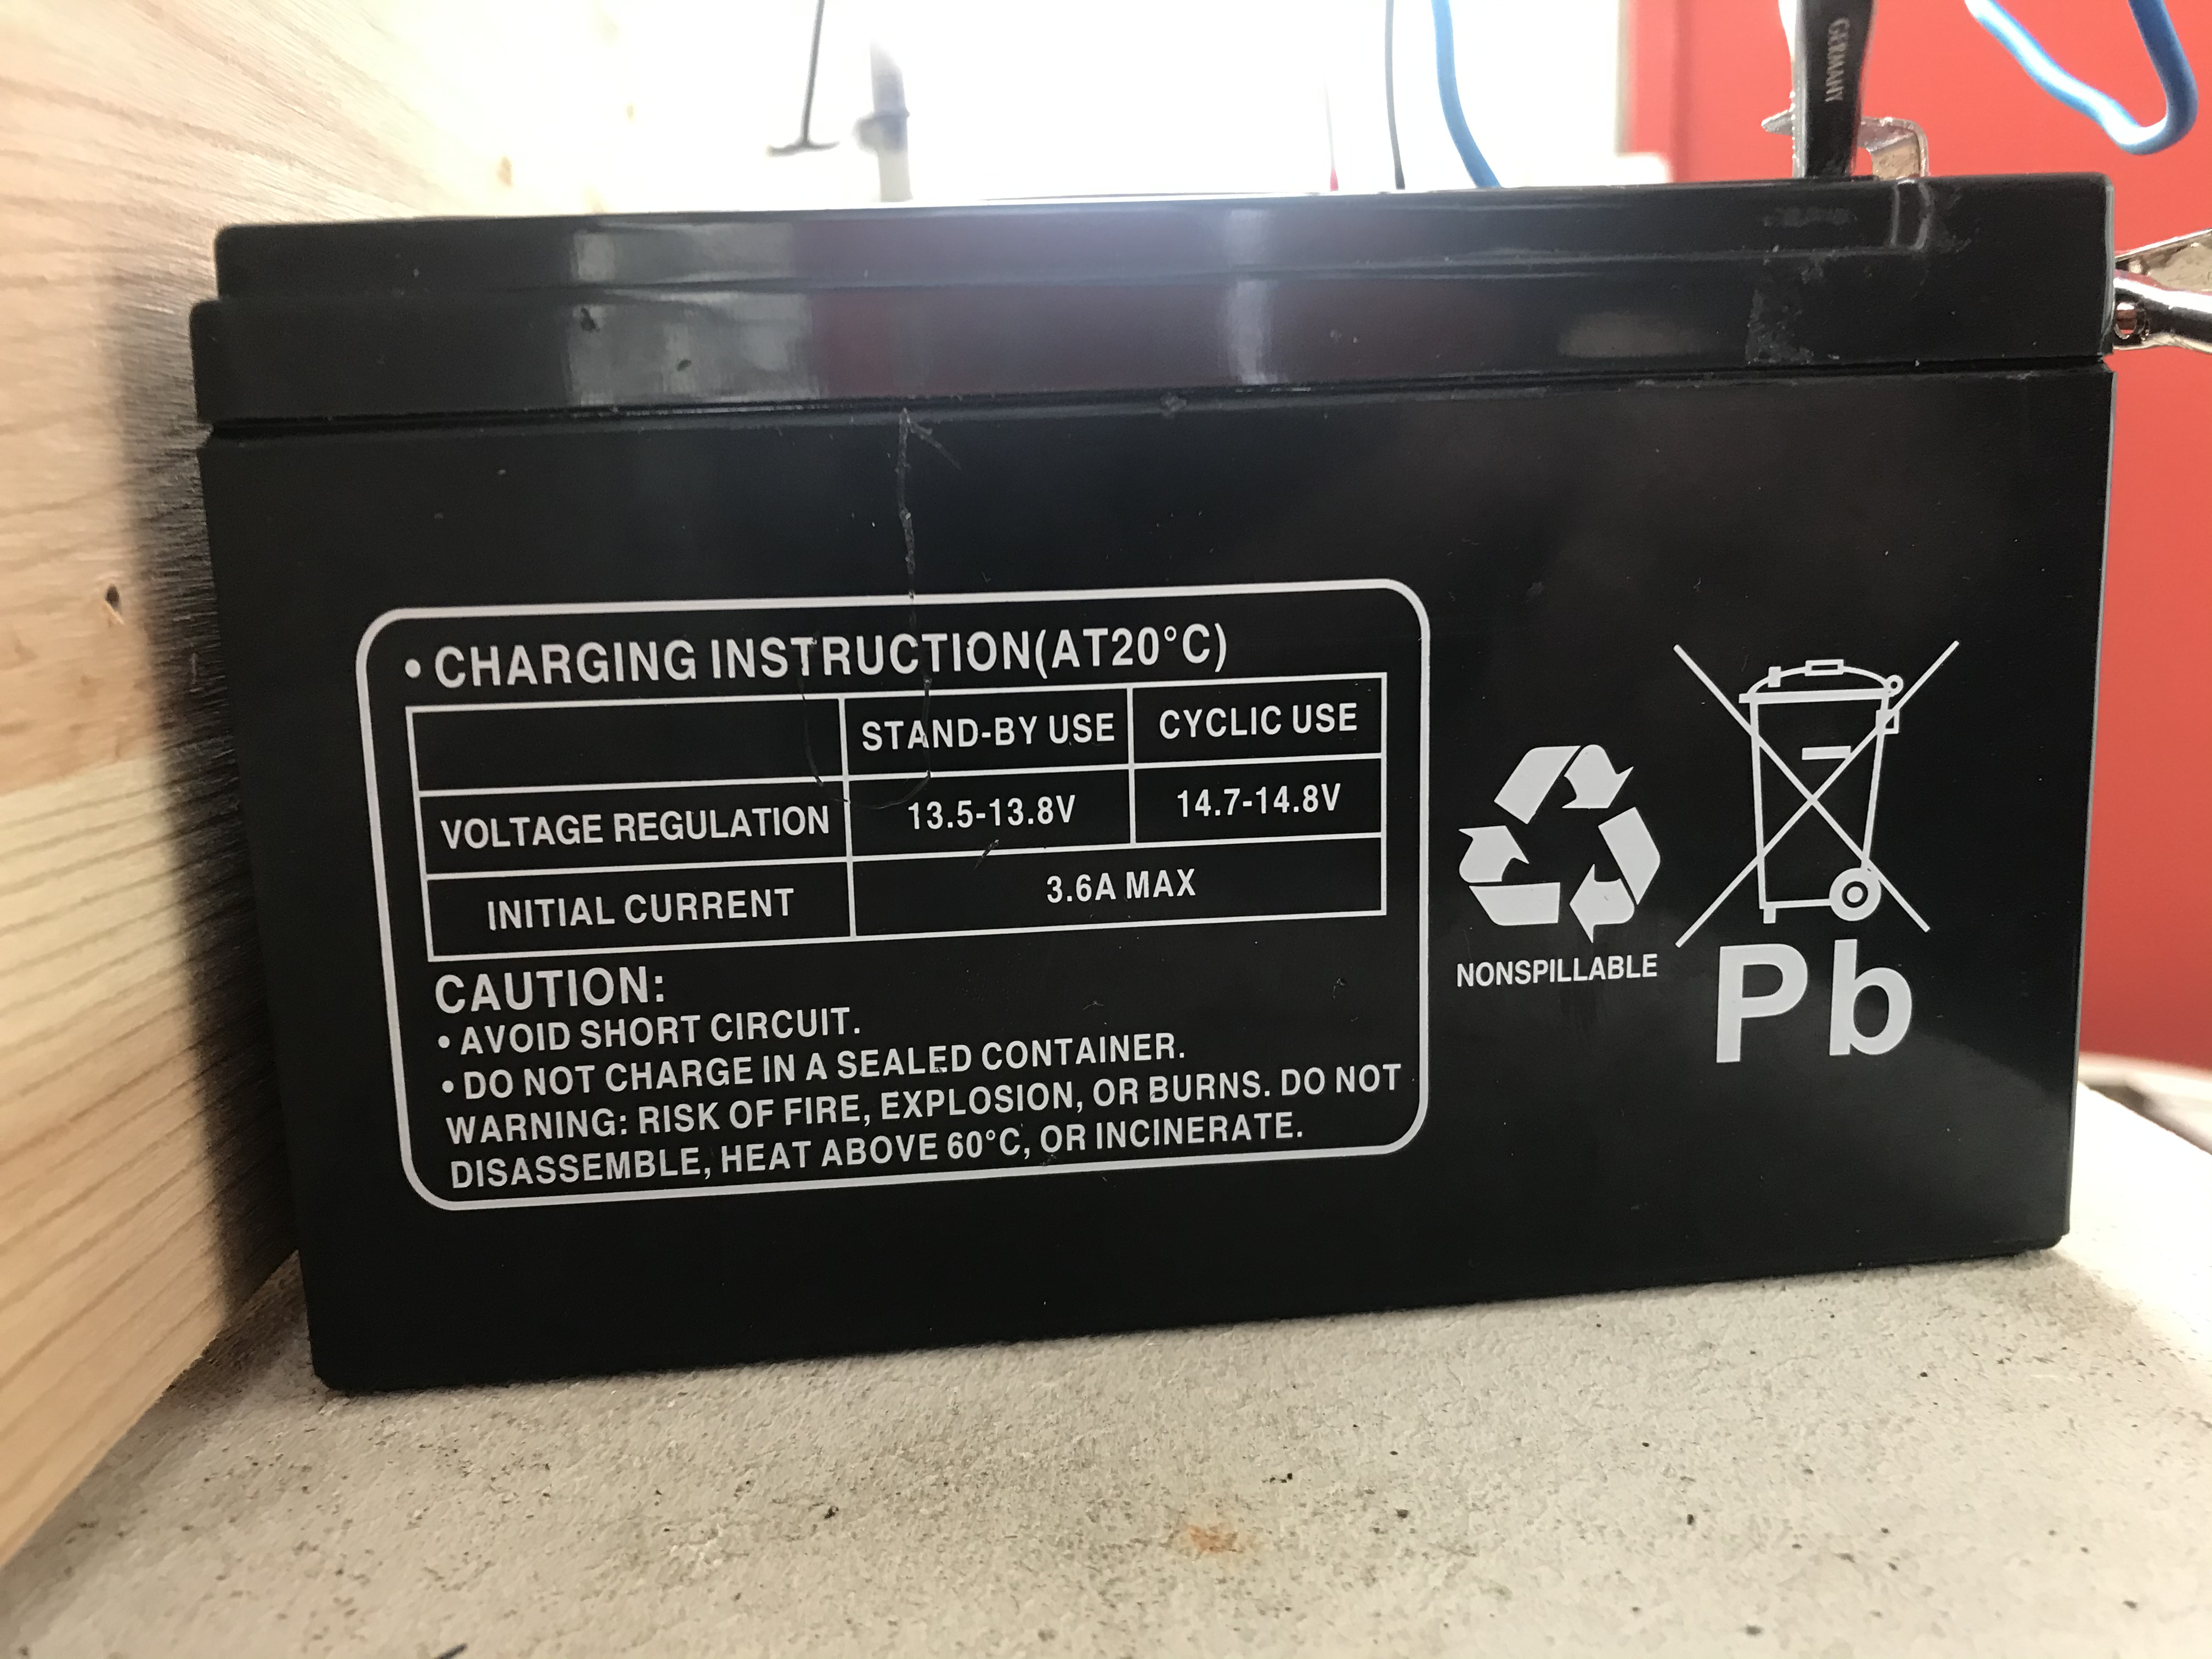
\includegraphics[width=.45\linewidth]{Bilder/Dokubilder/Batterie.jpg}}\hfill
\subfloat[Solar Laderegler]{\label{fig:Laderegler}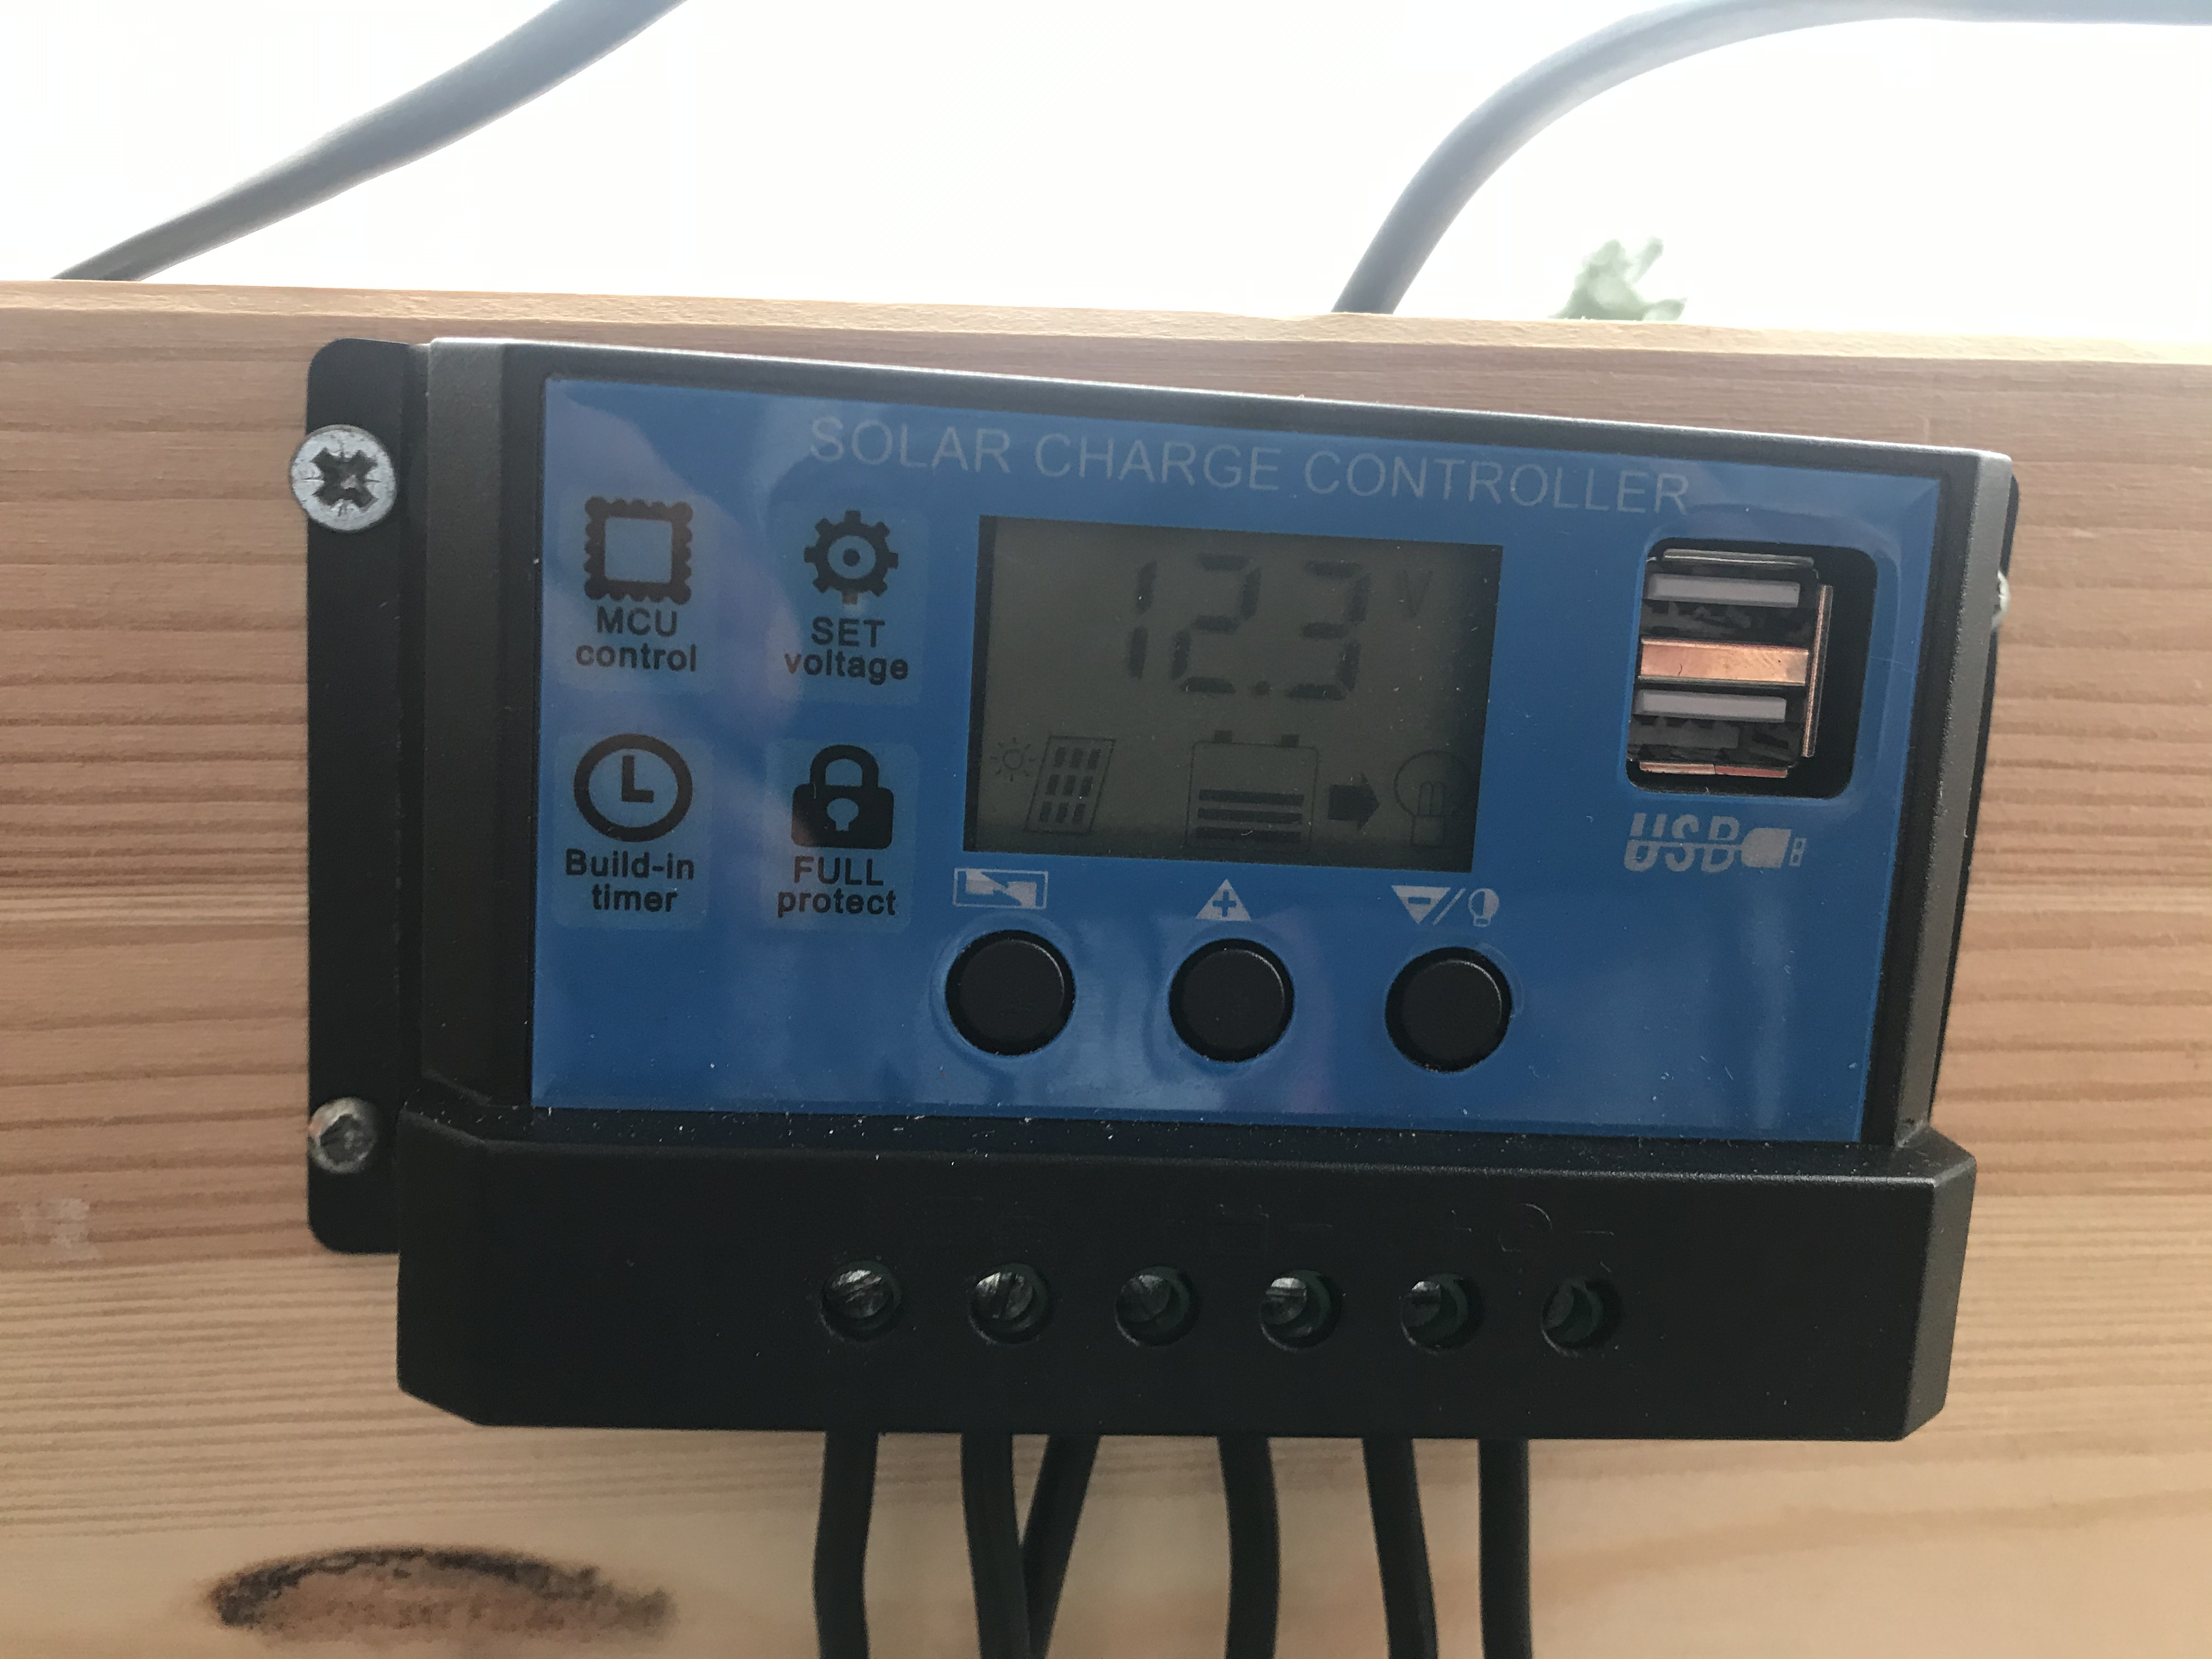
\includegraphics[width=.45\linewidth]{Bilder/Dokubilder/Controller.jpg}}\par 
\subfloat[PV Modul]{\label{fig:Solarmodul}\includegraphics[width=.45\linewidth]{Bilder/Dokubilder/PVKlein.jpg}}
\caption{Bestandteile der Solaranlage}
\label{fig:Solaranlage Bestandteile}
\end{figure}


	Das Monitoring System kann an 4 Punkten einsetzen. Die Spannung des Photovoltaikmoduls sowie der Batterie können jeweils mit einem Spannungssensormodul gemessen werden. Und der Strom der Anlage kann über zwei ACS712 Strommesser abgegriffen werden. Durch eine optionale Sicherung und einem Schalter an der Batterie ist eine Entladung über Nacht ausgeschlossen. Als Problematisch hat sich jedoch die Strommessung an der Batterie erwiesen, wodurch auf eine Betrachtung der Batterie Messwerte zunächst ersteinmal verzichtet wurde. 

\begin{figure}
			\centering
			\includegraphics[width=1\linewidth]{Bilder/Dokubilder/MonitoringZerlegt.JPG}
			\caption{Monitoring System in seine Einzelteile zerlegt}
			\label{fig:Monitoring zerlegt}
		\end{figure}	
	
	
	 
\newpage
Nun wurde ein Monitoring System an die Batterie und die Solaranlage angeschlossen. 

Dieses Monitoring System besteht aus 4 Komponenten: Einem ACS712 zur Strommessung, einem Voltagesensor zur Spannungsmessung, einem OLED-Display zur beobachtung vor Ort und dem ESP32 Node MCU als Mikrocontroller.Die Schaltung des Monitoring Systems ist dem folgenden schaubild zu entnehmen \ref{fig:Monitoring Einheit}.
\\		
		Bevor der Endzustand des Monitoring Systems auf zwei abnehmbare Sensoren festgelegt wurde sollten es vier sein. Zwei für die Batterie und zwei für das Photovoltaikmodul. Doch nach mehreren versuchen die Batteriespannung abzuklemmen wurde die Strom und Spannungsmessung der Batterie aufgegeben. Ein Kurzschluss hat leider eine alte Schaltung zerschossen. Deswegen ist es dabei geblieben nur den Strom und die Spannung des Solarmoduls zu messen. Diese erfolgen wie oben genannt mit einem ACS712 für den Strom und einem Spannungsmessmodul für die Spannung.
\\
Durch den vorfall fällt natürlich die Strom-/Spaannungsmessung an der Batterie weg, sodass die Schaltskizze nun wie im folgenden Bild zu sehen aufgebaut ist\ref{fig: Schaltskizze Solaranlage neu}.

\begin{figure*}
    \begin{center}
    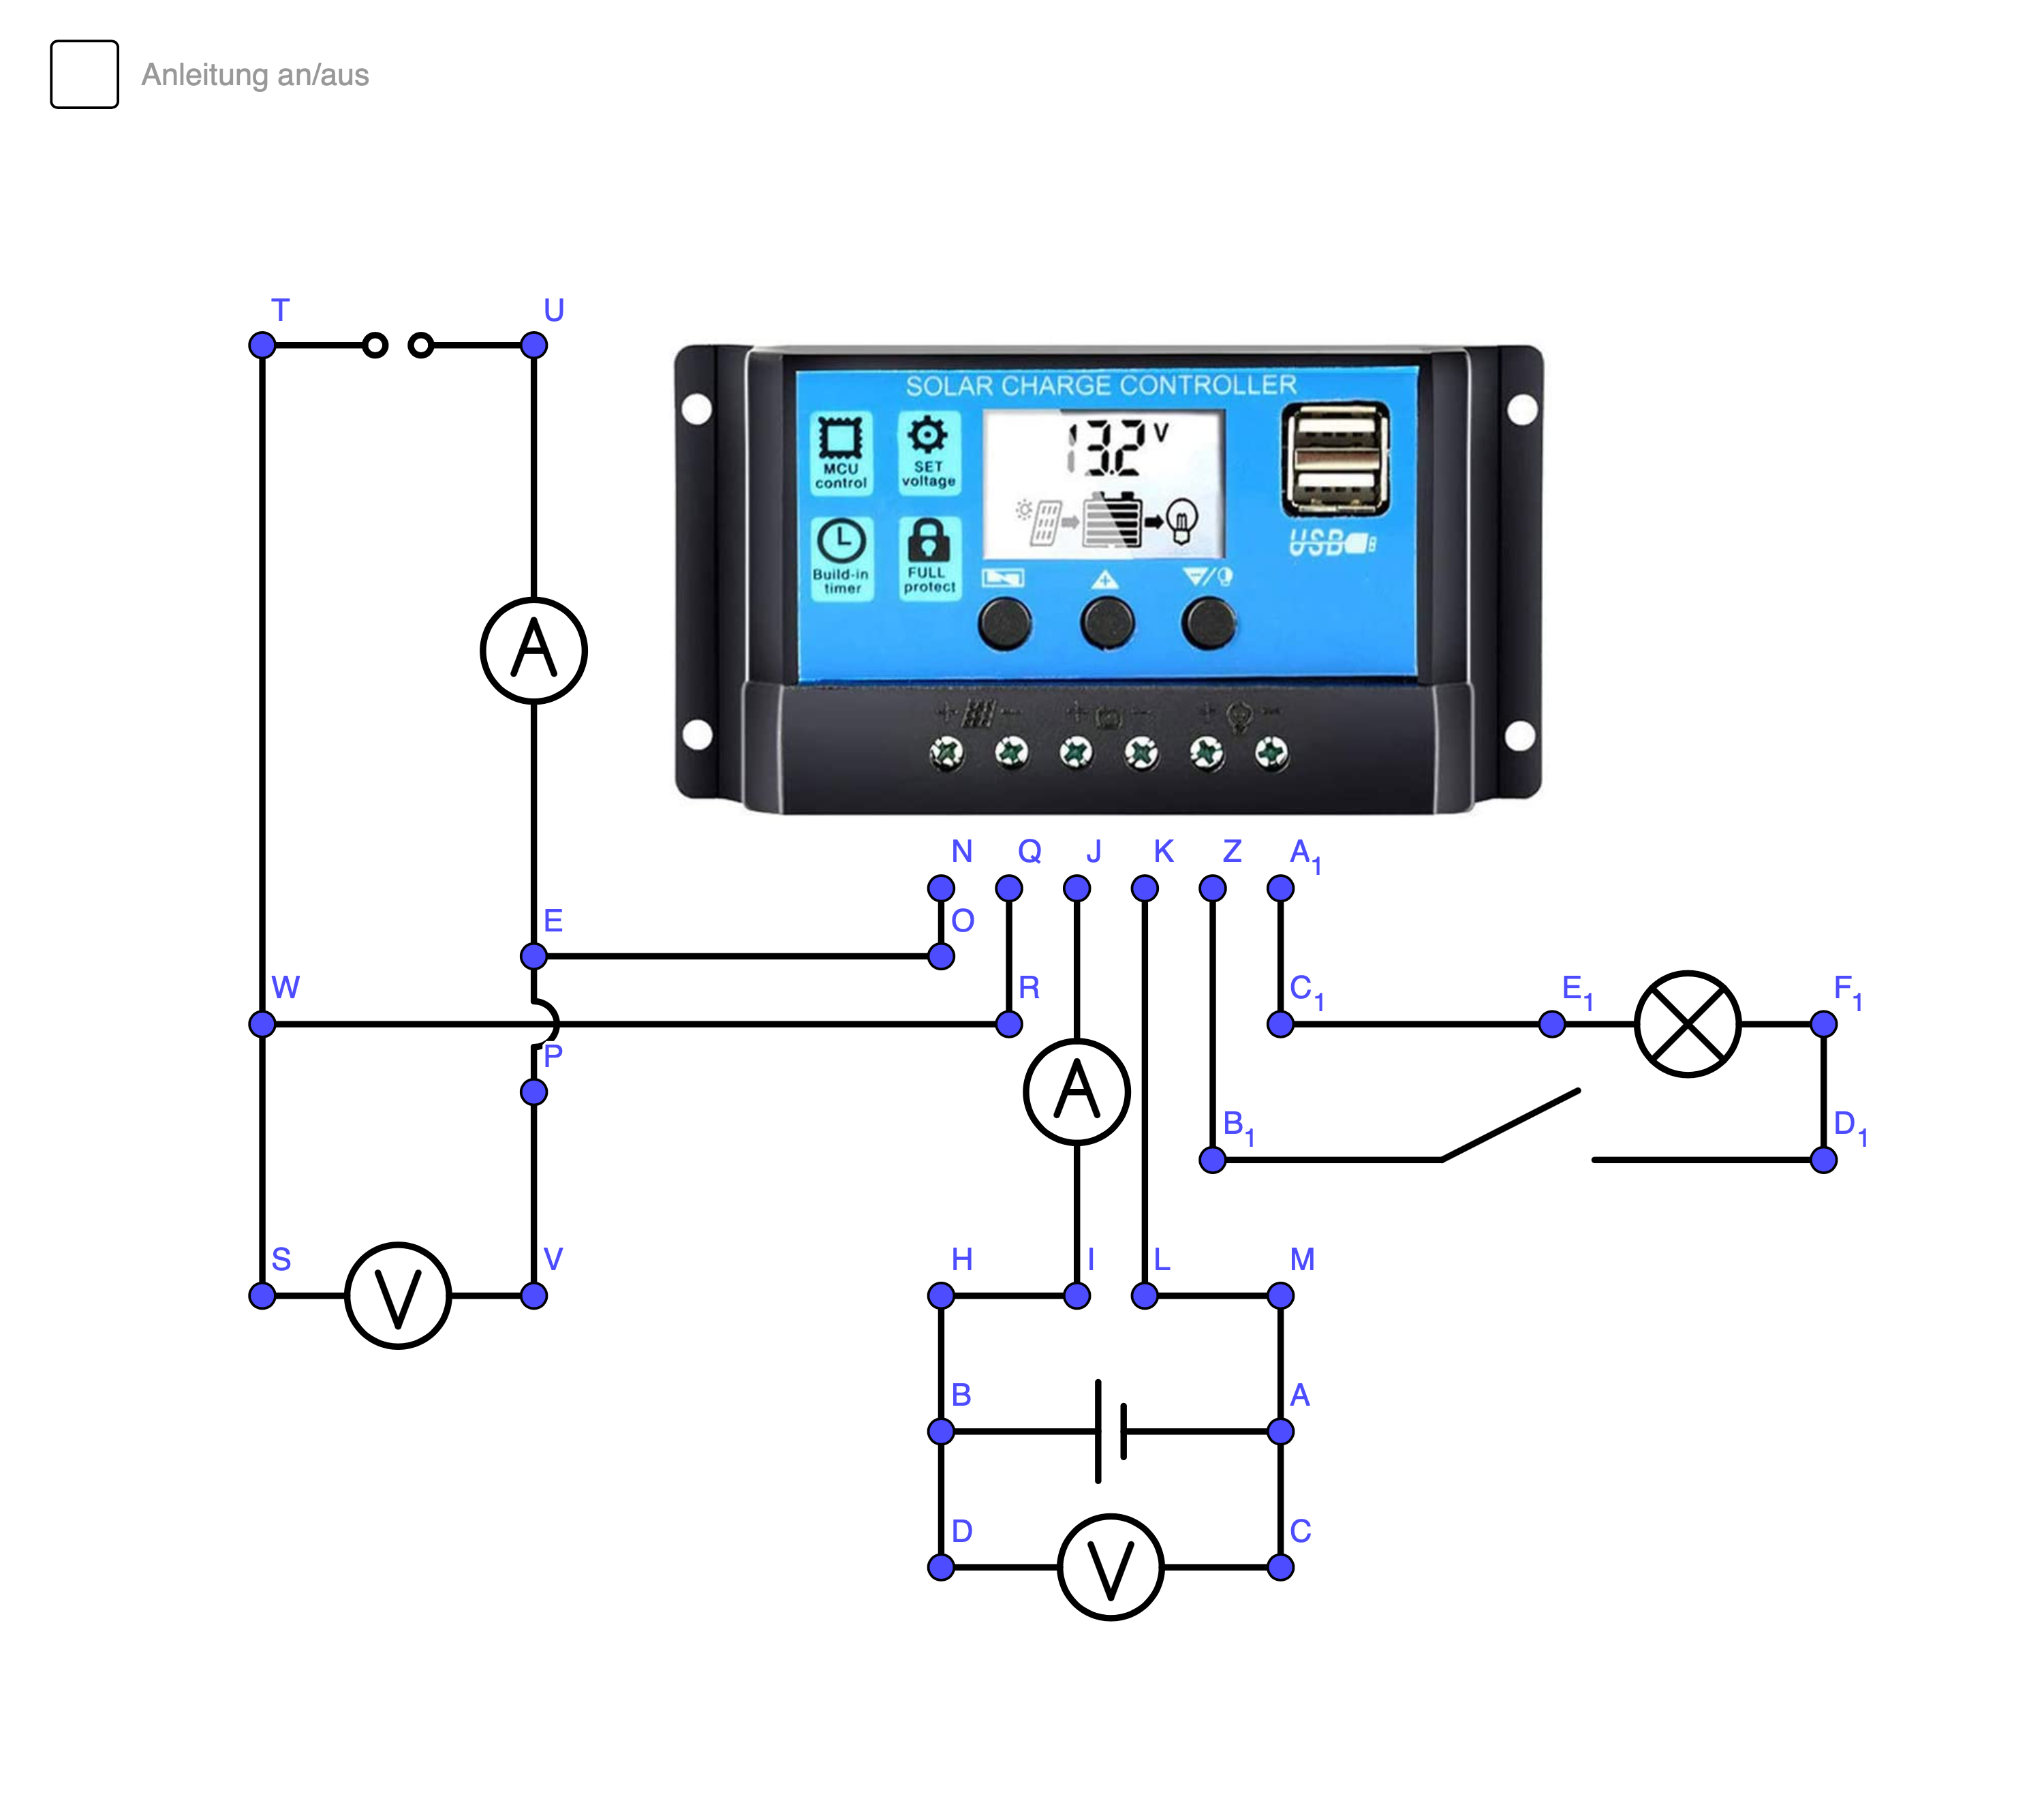
\includegraphics[width=\linewidth,height=.45\textheight,keepaspectratio]{Bilder/Schaltbilder/SchaltungAnlage.png}
    \caption{Schaltskizze der Solaranlage mit Batteriemessung}
      \label{fig: Schaltskizze Solaranlage alt}
    \end{center}
    \end{figure*}


    \begin{figure*}
    \begin{center}
    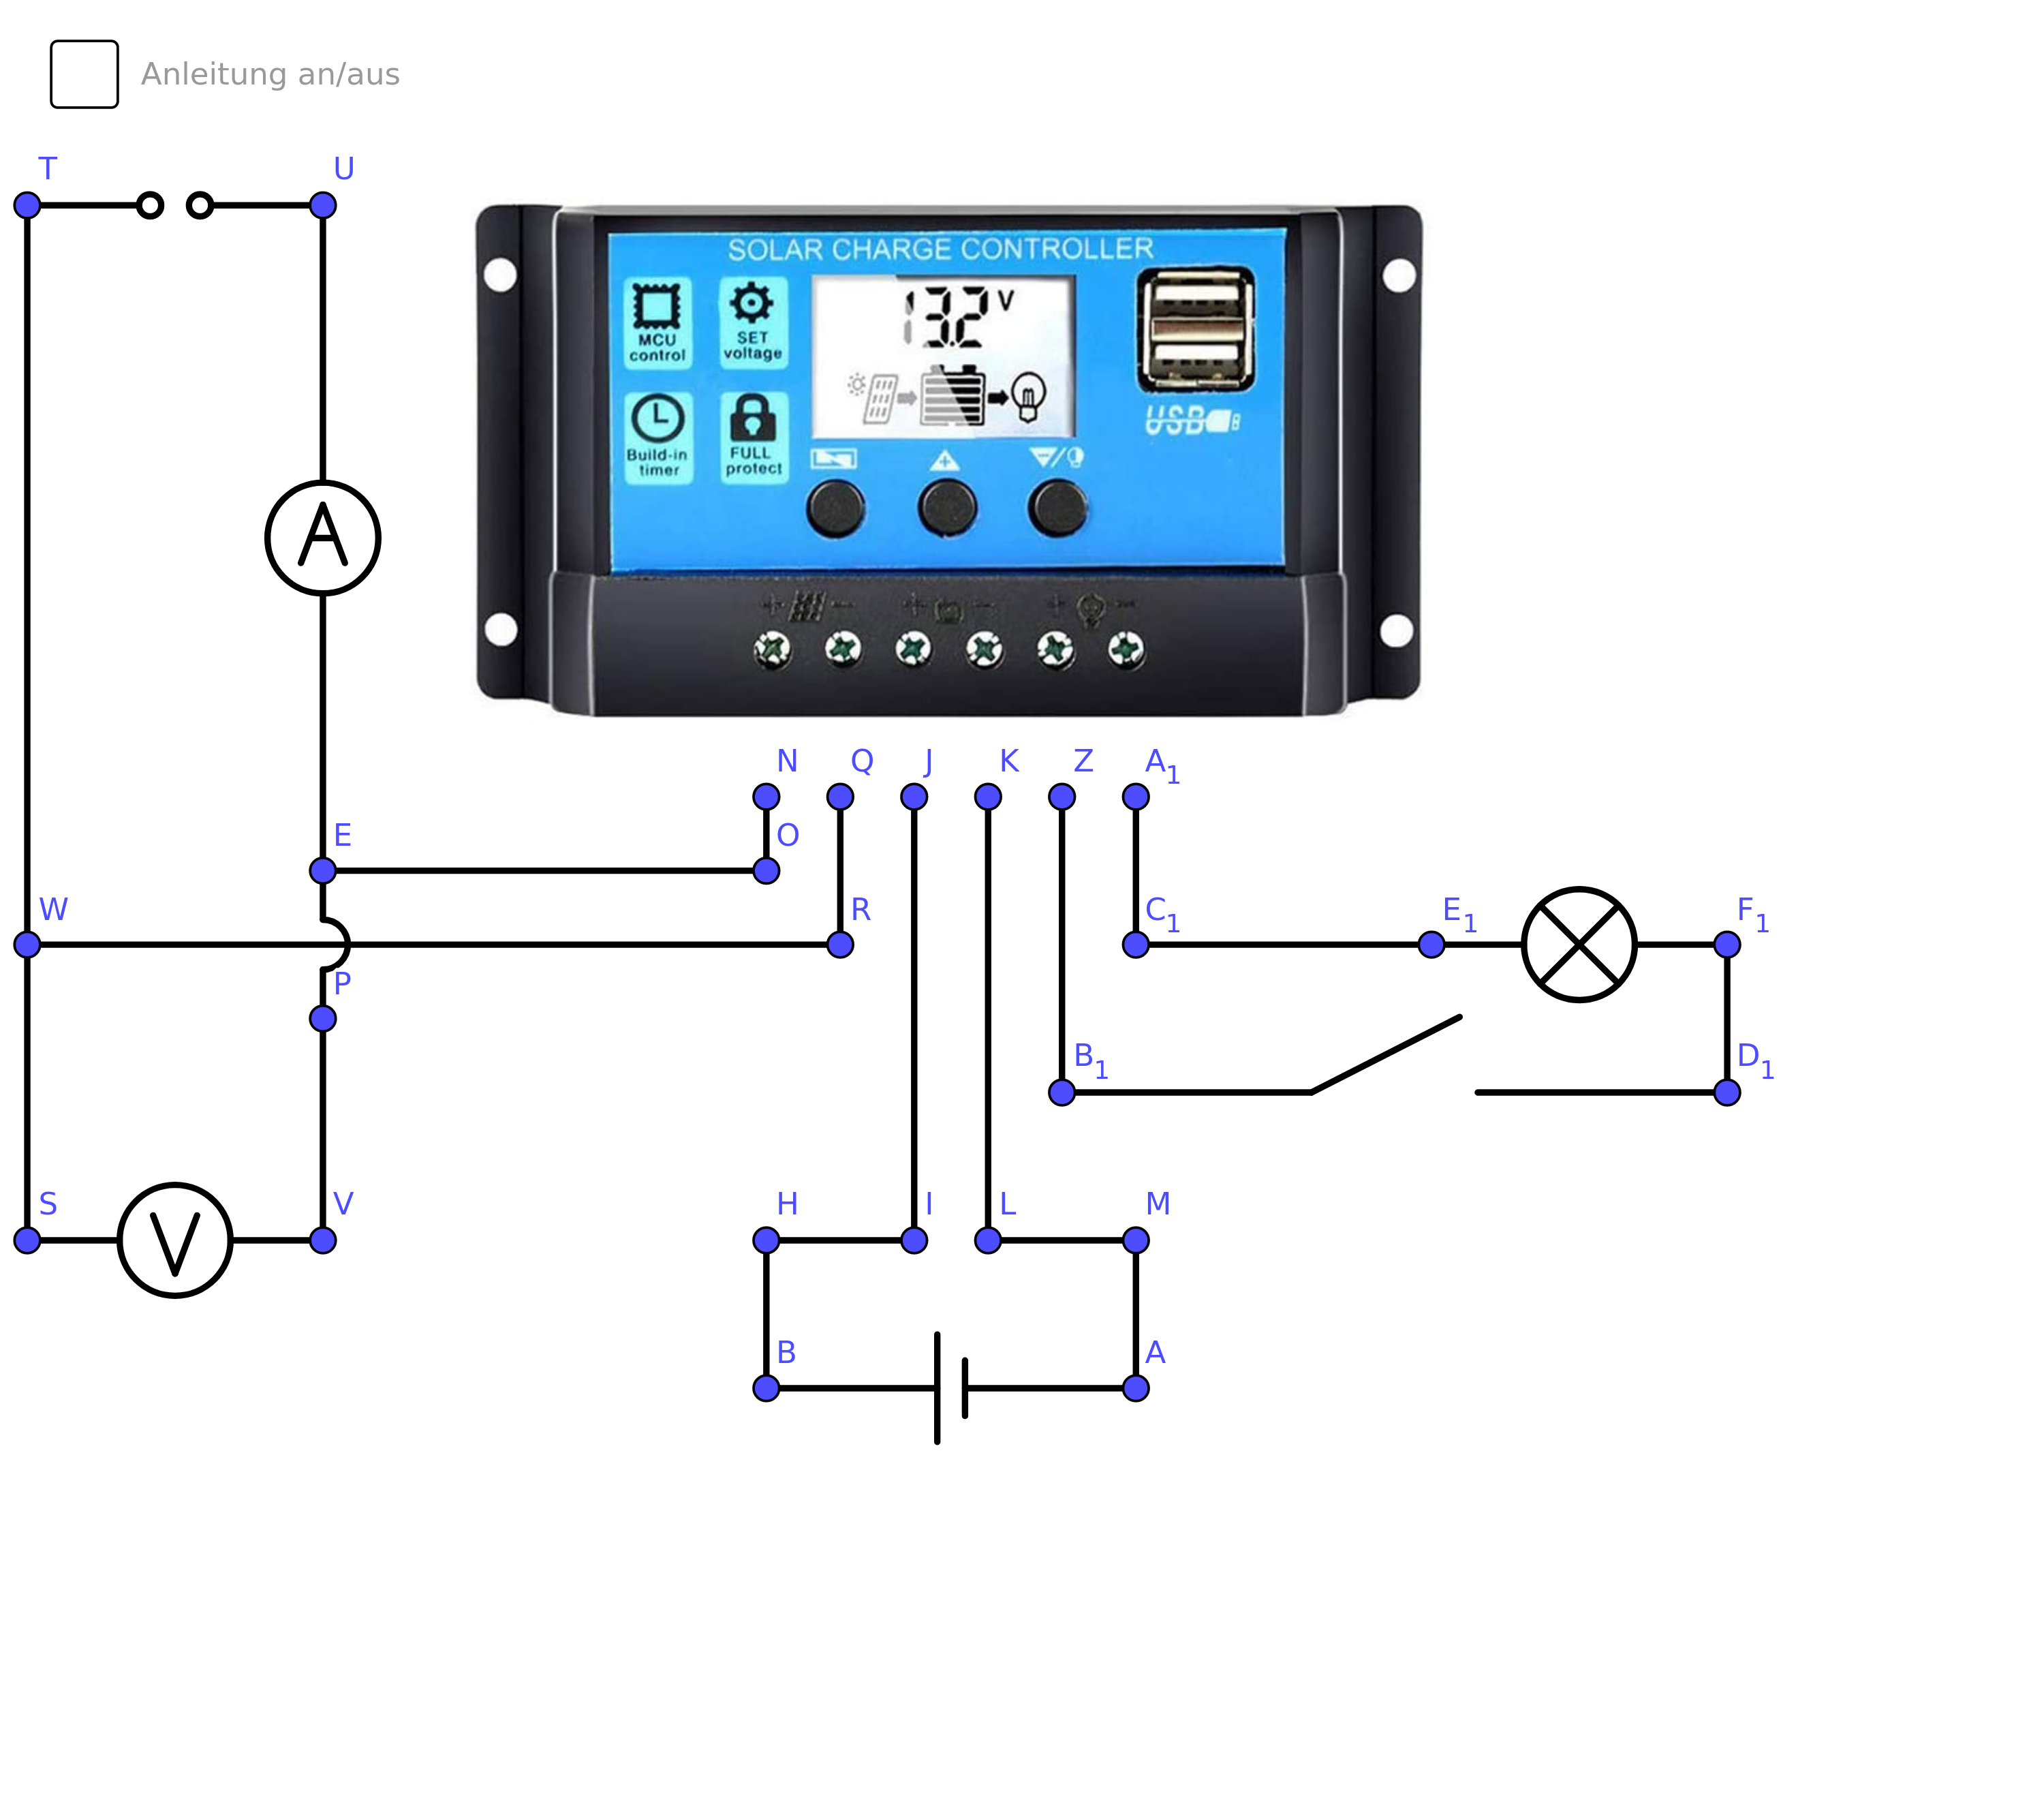
\includegraphics[width=\linewidth,height=.45\textheight,keepaspectratio]{Bilder/Schaltbilder/SchaltungOhneBatterieMessung.png}
    \caption{Schaltskizze der Solaranlage ohne Batteriemessung}
		\label{fig: Schaltskizze Solaranlage neu}
    \end{center}
    \end{figure*}
\newpage
\subsection{Schaltung}
Die Schaltung des Monitoring Systems ist der Abbildung \ref{fig:Monitoring Einheit} zu entnehmen.

		\begin{figure}
			\centering
			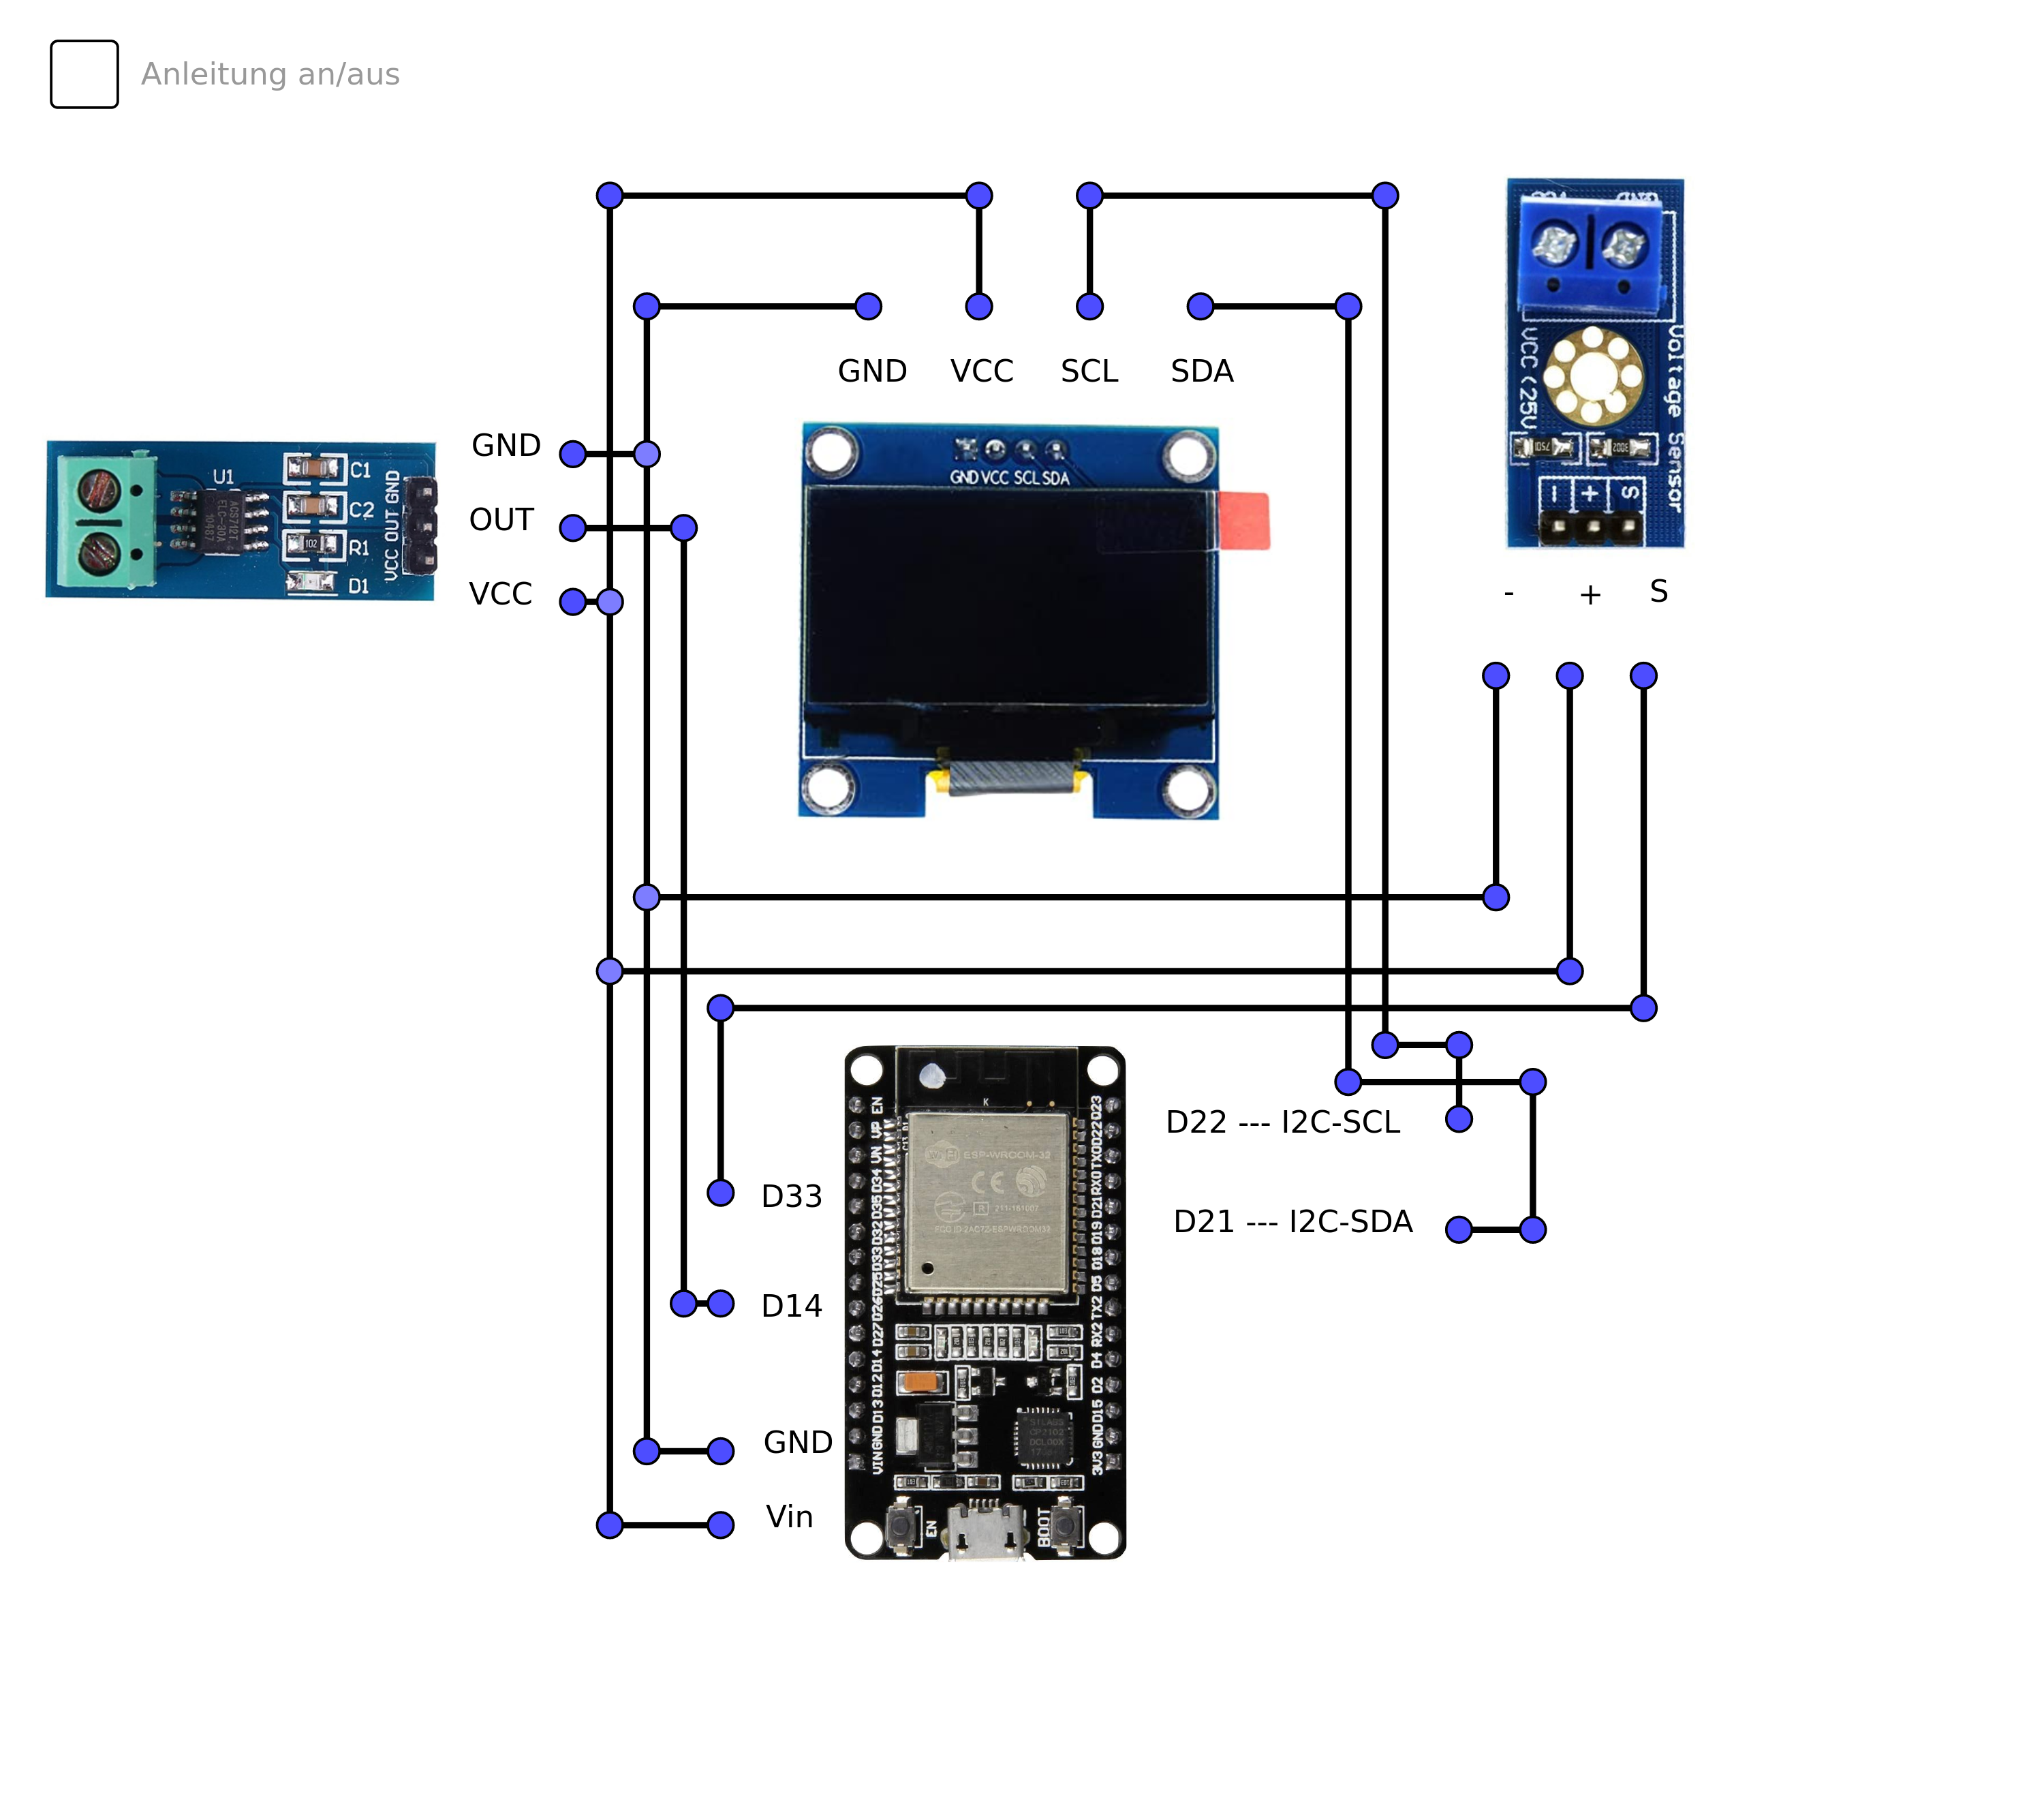
\includegraphics[width=1\linewidth]{Bilder/Schaltbilder/Monitoring_Schaltung.png}
			\caption{Schaltskizze der Monitoring Einheit}
			\label{fig:Monitoring Einheit}
		\end{figure}
		
Hier wurde der ESP32 NodeMcu an einen OLED-Display mit 1.3" geschlossen. Die Spannungsversorgung des OLED läuft über das $V_{IN}$ des ESP. Die Sensoren bekommen ihre Betriebsspannung auch aus dieser Quelle. Der SCK (clock Line) Pin\parencite{SPI.2021} ist an den Pin D22 des ESP angeschlossen. Der SDA (data Line) Pin\parencite{Wire.2021} ist an den Pin D21 des ESP angeschlossen. Die Sensoren sind jeweils mit Pin D14 für den Stromsensor und Pin D33 für den Spannungssensor verbunden.

Der wesentliche OLED Code ist im folgenden aufgeführt.

\begin{minted}[
frame=lines,
framesep=2mm,
baselinestretch=1.2,
bgcolor=LightGray,
fontsize=\footnotesize,
linenos
]{C++}
#include <SPI.h>
#include <Wire.h>
#include <Adafruit_GFX.h>
#include <Adafruit_SH1106.h>

#define OLED_SDA 21
#define OLED_SCL 22

Adafruit_SH1106 display(21, 22);

void setup()   {                
  Serial.begin(115200);
  /* initialize OLED with I2C address 0x3C */
  display.begin(SH1106_SWITCHCAPVCC, 0x3C); 
  display.clearDisplay();
  }

void loop() { 
  /* set text size, color, cursor position, 
  set buffer with  Hello world and show off*/
  display.setTextSize(2);
  display.setTextColor(WHITE);

display.setCursor(0,0);
  display.print("P= ");
  display.print(solarPower);
  display.print(power);
  
  display.setCursor(0,20);
  display.print("U= ");
  display.print(solarVoltage);
  display.print(voltage);
  display.print(" ");
  
  display.setCursor(0,40);
  display.print("I= ");
  display.print(solarCurrent);
  display.print(ampere);

  display.display();
  delay(100);
  display.clearDisplay();
}

\end{minted}
\newpage


%%%%%%%%%%%%%%%%%%%%%%%%%%%%%%%%%%%%%%%%%%%%%%%%%%%%%%%%%%%%%%%%%%%%%%
\subsection{code}

Der Programmcode besteht aus zwei Bestandteilen. Zum einen dem Sketch für den Arduino und zum anderen dem HTML-Code für den Webserver.

\textbf{Arduino Code}

Die folgenden Bibliotheken sind bestandteil der Anwendung. Darunter die SPI (für SCK), Wire (für SDA) und die beiden Adafruit Bibliotheken zur Kommunikation mit dem I2C Oled Display.\parencites{SPI.2021}{Wire.2021}.
Die Spiffs Bibliothek um die index.html Datei des Webservers in HTML und CSS in der Flash Memory der ESP32 zu laden\parencites{SPIFFS.2021}. Und die letzten beiden Bibliotheken WIFi und ESPAsyncWebServer um einen Web Server auf dem port 80 des ESP32 zu generieren.

\begin{minted}[
frame=lines,
framesep=2mm,
baselinestretch=1.2,
bgcolor=LightGray,
fontsize=\footnotesize,
linenos
]{C++}
#include <SPI.h>
#include <Wire.h>
#include <SPIFFS.h>
#include <Adafruit_GFX.h>
#include <Adafruit_SH1106.h>
#include <WiFi.h>
#include <ESPAsyncWebServer.h>
\end{minted}

Daraufhin werden die Sensor Pins deklarier, wobei der Pin D33 [ADC5] des ESP an den Sensor Pin des Spannungsmesser angeschlossen wird und der Pin 14 [ADC16] an den ACS712. Die folgenden Attribute vOut und vIN dienen dem Spannungsmesseralgorithmus zur bestimmung der anliegenden Solarspannung. R1 und R2 sind die Widerstände auf dem Spannungsmesser die in einen Spannungsteiler geschaltet sind. Siehe \ref{fig:Spannungsteiler}.

		\begin{figure}
			\centering
			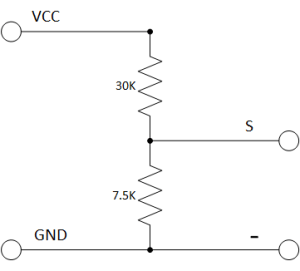
\includegraphics[scale=.5]{Bilder/Dokubilder/voltageSensorSpannungsteiler.jpg}
			\caption{Spannungsteiler des Spannungsmessers}
			\label{fig:Spannungsteiler}
		\end{figure}

\begin{minted}[
frame=lines,
framesep=2mm,
baselinestretch=1.2,
bgcolor=LightGray,
fontsize=\footnotesize,
linenos
]{C++}
const int voltageSensor = 33;
const int currentSensor = 14;

float vOUT;
float vIN;

float R1 = 30000.0;
float R2 = 7500.0;

\end{minted}

Im folgenden sind die drei Methoden aufgeführt um die Spannung, den Strom und die Leistung des Solarmoduls zu berechnen. Bei der Spannunsmessung wird der am Sensor über ein analogRead eingelesene wert über die 12 Bit Auflösung des ADC Pins in 4095 Werte unterteilt, wobei die $3.9V$ die Richtspannung des ESP32 am $V_{in}$ ist. Im folgenden wird über den Spannungsteiler die angelegte Spannung ermittelt. Diese Methode liefert die angelegte Spannung zurück. 


\begin{figure}
			\centering
			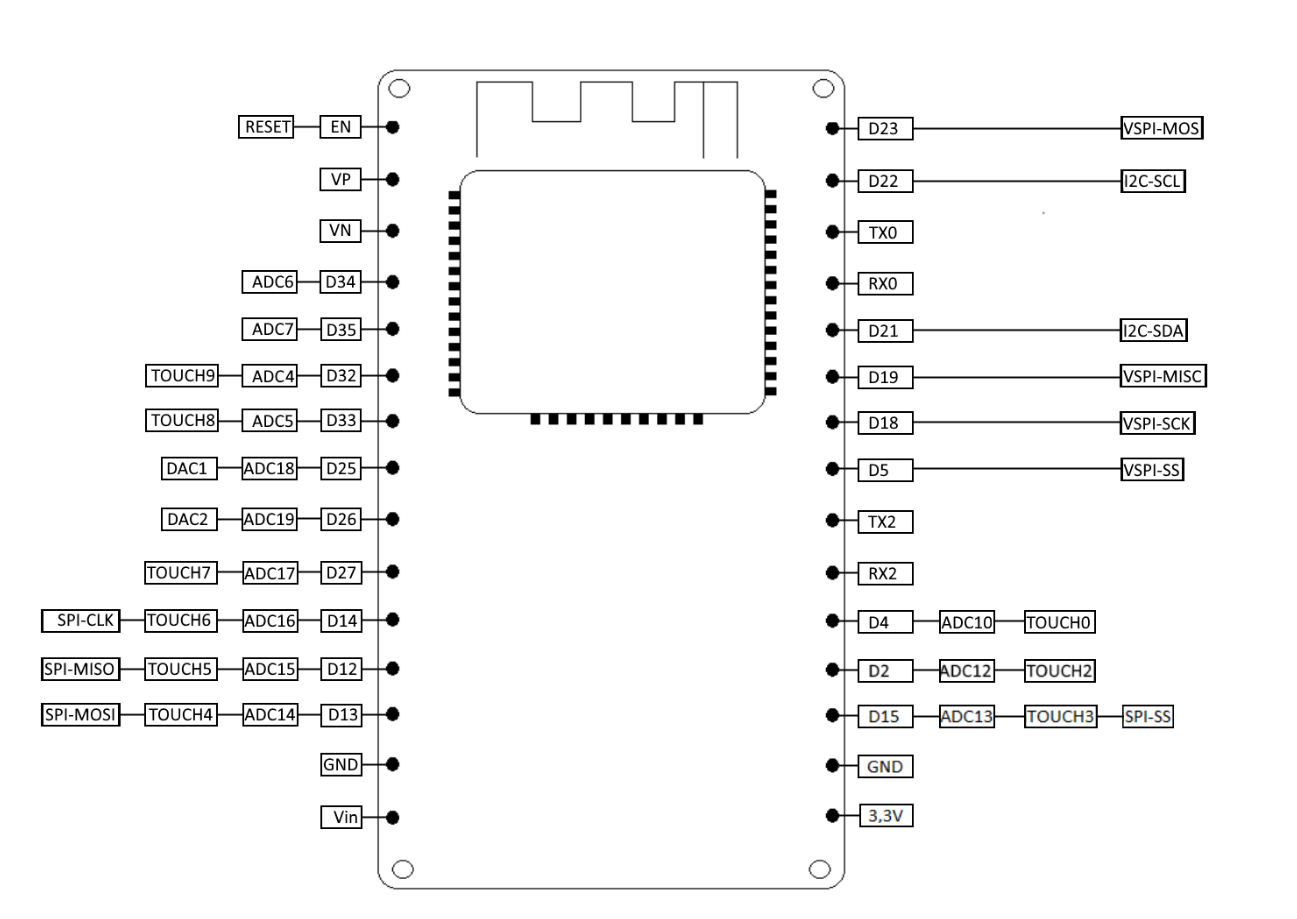
\includegraphics[scale=.3]{Bilder/Dokubilder/esp32.png}
			\caption{Pinout des ESP32 NodeMCU}
			\label{fig:Pinout ESP32}
		\end{figure}


\begin{minted}[
frame=lines,
framesep=2mm,
baselinestretch=1.2,
bgcolor=LightGray,
fontsize=\footnotesize,
linenos
]{C++}
float spannungsmessung(){
  value = analogRead(voltageSensor);
  vOUT = (value * 3.9) / 4096.0;
  vIN = vOUT / (R2/(R1+R2));
  solarVoltage = vIN;
  delay(50);
  return solarVoltage;
}
\end{minted}

Im folgenden wird die Methode zur bestimmung der Stromstärke näher erläutert. Diese bildet zunächts den Mittelwert über 150 Messwerte und unterteilt diesen wieder auf 4096 Werte. Zudem wird eine Abweichung von 2.5 Subtrahiert und durch den Messfehler des 20A ACS712 dividiert. Schlussendlich habe ich eine kleine korrektur vorgenommen um den solarCurrent-Wert in $mA$ ausgeben zu können. Diese Methode liefert den Strom der durch das Modul fließt zurück. 

\begin{minted}[
frame=lines,
framesep=2mm,
baselinestretch=1.2,
bgcolor=LightGray,
fontsize=\footnotesize,
linenos
]{C++}

float strommessung() {
unsigned int x=0;
float AcsValue=0.0,Samples=0.0,AvgAcs=0.0,AcsValueF=0.0;

  for (int x = 0; x < 150; x++){ 
  AcsValue = analogRead(currentSensor);        
  Samples = Samples + AcsValue;  
  delay (3); 
}
AvgAcs = Samples/150.0;

AcsValueF = (2.5 - (AvgAcs * (3.925 / 4096.0)) )/0.185;
solarCurrent = AcsValueF*(-10);
delay(50);
return solarCurrent;
}
\end{minted}

Um den Leistungswert des Moduls zu bestimmen bildet diese Methode das Produkt aus der Spannung und der Stromstärke die am Modul anliegt.

\begin{minted}[
frame=lines,
framesep=2mm,
baselinestretch=1.2,
bgcolor=LightGray,
fontsize=\footnotesize,
linenos
]{C++}
float leistungsBerechnung(){
  solarPower = solarVoltage*(solarCurrent/1000);
  return solarPower;
}
\end{minted}



%%%%%%%%%%%%%%%%%%%%%%%%%%%%%%%%%%%%%%%%%%%%%%%%%%%%%%%%%%%%%%%%%%%%%%
\subsection{Drahtlose Übertragung}

Die Drahtlose Übertragung wird über zwei Dateien realisiert. Mit dem Arduino Sketch und einer HTML Datei mit css.


\begin{figure}
			\centering
			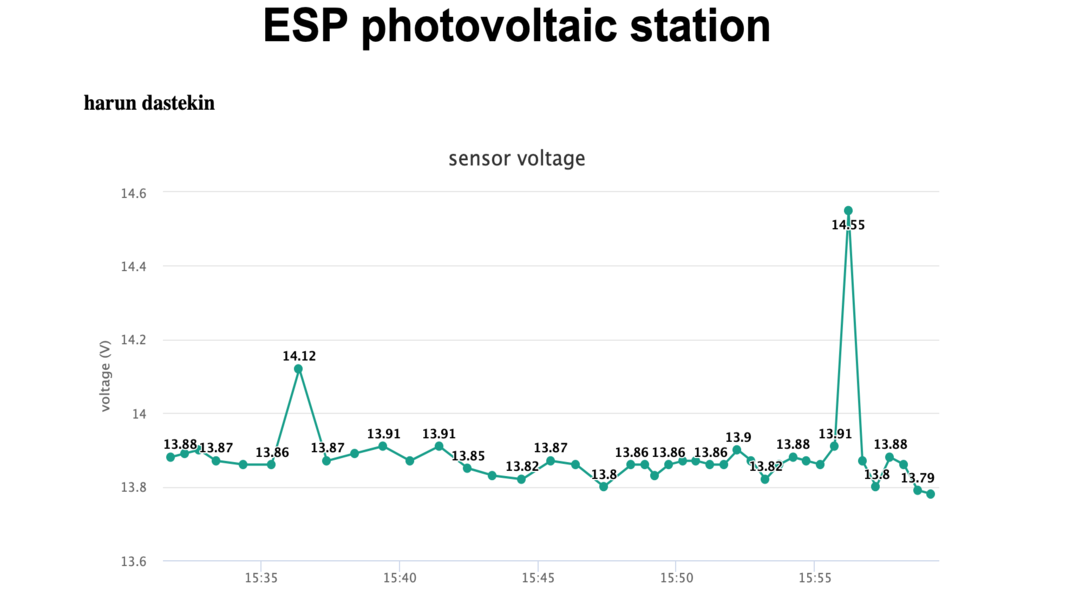
\includegraphics[width=1\linewidth]{Bilder/Dokubilder/WebServer.png}
			\caption{Web Server ausschnitt für den Spannungsmesser}
			\label{fig:Web Server}
		\end{figure}


Die übertragung der Messwerte der Solaranlage über den ESP32 an den Web Server erfolgt über Wifi. Dazu wird eine HTML Datei in den Flash Speicher des ESP über einen SPIFF upload mihilfe des Arduino ESP32 Filesystem Uploaders\parencite{SPIFFS.2021}.
\\
Mithilfe der Zugangsdaten für das Wifi-Netz wird ein Asynchroner Web Server auf dem Port 80 gestartet.

\begin{minted}[
frame=lines,
framesep=2mm,
baselinestretch=1.2,
bgcolor=LightGray,
fontsize=\footnotesize,
linenos
]{C++}

// Replace with your network credentials
const char* ssid = "Okily_Dokily";
const char* password = "Diablo0704..e-H!88";

// Create AsyncWebServer object on port 80
AsyncWebServer server(80);

\end{minted}

Im void setup der Anwendung wird nach dem seriellen Übertragung mit einer Baudrate von 115200, der OLED angesteuert. Da es sich hierbei um einen I2C mit 1.3" mit 128x64 pixel ist wird hier mit 0x3C initialisiert\parencite{OLEDCode.2020}. Nach dem clearDisplay erfolgt der SPIFFS verbindungsaufbau. Hiernach erfolgt der Wifi verbindungsaufbau und die Ausgabe der IP-Adresse des Netzes.

\begin{minted}[
frame=lines,
framesep=2mm,
baselinestretch=1.2,
bgcolor=LightGray,
fontsize=\footnotesize,
linenos
]{C++}
void setup()   {                
  Serial.begin(115200);
  display.begin(SH1106_SWITCHCAPVCC, 0x3C); 
  display.clearDisplay();

if(!SPIFFS.begin()){
  Serial.println("Fehler bei SPIFF connection");
  while(1);
}

// Connect to Wi-Fi
  WiFi.begin(ssid, password);
  while (WiFi.status() != WL_CONNECTED) {
    delay(1000);
    Serial.println("Connecting to WiFi..");
  }

// Print ESP32 Local IP Address
  Serial.println(WiFi.localIP());
\end{minted}

Im weiteren verlauf des void setup werden HTTP GET request routen festgelegt und der Server gestartet.

\begin{minted}[
frame=lines,
framesep=2mm,
baselinestretch=1.2,
bgcolor=LightGray,
fontsize=\footnotesize,
linenos
]{C++}

// Route for root / web page
  server.on("/", HTTP_GET, [](AsyncWebServerRequest *request){
    request->send(SPIFFS, "/index.html");
  });
  server.on("/voltage", HTTP_GET, [](AsyncWebServerRequest *request){
    request->send_P(200, "text/plain", readVoltage().c_str());
  });
  server.on("/current", HTTP_GET, [](AsyncWebServerRequest *request){
    request->send_P(200, "text/plain", readCurrent().c_str());
  });
  server.on("/power", HTTP_GET, [](AsyncWebServerRequest *request){
    request->send_P(200, "text/plain", calculatePower().c_str());
  });

  // Start server
  server.begin();
}
\end{minted}

Zunächst wird die Highcharts Bibliothek importiert \parencite{Highcharts.2021} um ein interaktives Diagramm zu nutzen.

\begin{minted}[
frame=lines,
framesep=2mm,
baselinestretch=1.2,
bgcolor=LightGray,
fontsize=\footnotesize,
linenos
]{HTML}
<script src="https://code.highcharts.com/highcharts.js"></script>
\end{minted}

Dann werden für die einzelnen Graphen jeweils eigene Content Division element (<div>) mit einer je eigenen id erzeugt.

\begin{minted}[
frame=lines,
framesep=2mm,
baselinestretch=1.2,
bgcolor=LightGray,
fontsize=\footnotesize,
linenos
]{HTML}
	<div id="chart-voltage" class="container"></div>
    <div id="chart-current" class="container"></div>
    <div id="chart-power" class="container"></div>
\end{minted}

Um Graphen zu generieren und Datenpunkte auf Ihnen zu setzen wird javascript genutzt. Der Folgende Code Snippet legt den Titel, die Achsen, die Farben usw. fest.

\begin{minted}[
frame=lines,
framesep=2mm,
baselinestretch=1.2,
bgcolor=LightGray,
fontsize=\footnotesize,
linenos
]{HTML}
var chartT = new Highcharts.Chart({
        chart: { renderTo: 'chart-voltage' },
        title: { text: 'sensor voltage' },
        series: [{
            showInLegend: false,
            data: []
        }],
        plotOptions: {
            line: {
                animation: false,
                dataLabels: { enabled: true }
            },
            series: { color: '#059e8a' }
        },
        xAxis: {
            type: 'datetime',
            dateTimeLabelFormats: { second: '%H:%M:%S' }
        },
        yAxis: {
            title: { text: 'voltage (V)' }
        },
        credits: { enabled: false }
\end{minted}

Schlussendlich fügt die setIntervall Methode dem Graphen Punkte hinzu und schickt alle 30 Sekunden ein GET - request an die /voltage URL um die Spannungswerte des ESP zu bekommen. Die anderen Graphen werden demetsprechend angesprochen.

\begin{minted}[
frame=lines,
framesep=2mm,
baselinestretch=1.2,
bgcolor=LightGray,
fontsize=\footnotesize,
linenos
]{HTML}
	setInterval(function () {
        var xhttp = new XMLHttpRequest();
        xhttp.onreadystatechange = function () {
            if (this.readyState == 4 && this.status == 200) {
                var x = (new Date()).getTime(),
                    y = parseFloat(this.responseText);
               
                if (chartT.series[0].data.length > 40) {
                    chartT.series[0].addPoint([x, y], true, true, true);
                } else {
                    chartT.series[0].addPoint([x, y], true, false, true);
                }
            }
        };
        xhttp.open("GET", "/voltage", true);
        xhttp.send();
    }, 30000);
\end{minted}


\section{Fazit und Ausblick}
In Zukunft möchte ich gerne ein Mppt-Regler bauen der drei Zustände besitzt\parencite{Electronoobs.2020}. Den "Bulk-Modus" der eine konstante Stromstärke liefert um die Batterie bis auf 80\% zu laden (ohne rücksicht auf die Spannung zu nehmen). Ab einer bestimmten Spannung der Batterie soll der nächste Zustand einsetzen "Absorption". Hier bleibt die Spannung durch den Controller konstant, die Stromstärke nicht mehr, diese fällt mit dem Ladezustand der Batterie (nahe 100\%). Dann sobald die Batterie die restlichen 20\% geladen hat soll der Controller in den "Float"-Modus. In diesem Zustand reduziert der Controller die Spannung auf einen festgesetzten Wert und der Stromfluss reduziert sich auf einen Wert kleiner als 1\% der Batterie Kapazität. Dadurch kann die Batterie unendlich lange voll geladen bleiben. Ein Bild dieser Idee sieht man auf der folgenden Abbildung\ref{fig:MPPT Solar Charger Prototype}.

\begin{figure}
			\centering
			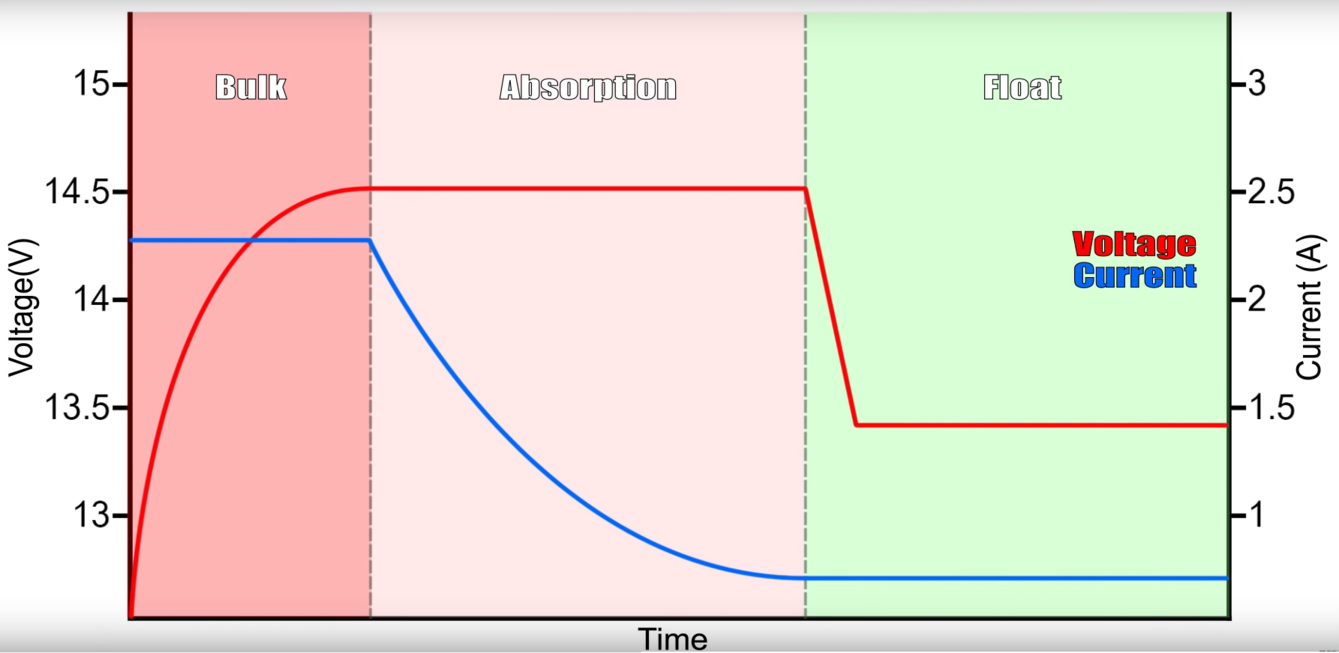
\includegraphics[width=1\linewidth]{Bilder/Dokubilder/ChargeController1.png}
			\caption{Ladekurve der Mppt-Controller Idee}
			\label{fig:MPPT Solar Charger Prototype}
		\end{figure}


Ich habe einen solchen Versuch gestartet. Nach einigen durchgebrannten Schaltungen und fehlenden Teilen habe ich diesen Versuch eingefroren. 


\begin{figure}
		\centering
		\includegraphics[width=1\linewidth]{Bilder/Dokubilder/Anlage.jpg}
		\caption{Anlage in Konstruktion}
		\label{fig:Solaranlage}
	\end{figure}

\newpage



%Abbildungsverzeichnis
\listoffigures \clearpage

\printbibliography

% Anhang
\newpage
\section{\textbf{Anhang}}

\textbf{Arduino Code}
\lstinputlisting[language=C++,
basicstyle=\scriptsize,linerange={1,17-42},
numbers=left,numberstyle=\tiny,stepnumber=2,numbersep=5pt,
frame=single, framerule=1pt
]{code/monitoringCode/monitoringCode.ino}

\textbf{Webserver Code}
\lstinputlisting[language=HTML,
basicstyle=\scriptsize,linerange={1,17-42},
numbers=left,numberstyle=\tiny,stepnumber=2,numbersep=5pt,
frame=single, framerule=1pt
]{code/monitoringCode/data/index.html}

\includepdf[pages=1-6]{Quellen/SBC-NodeMCU-ESP32-Anleitung-20200320.pdf}
\includepdf[pages=1-15]{Quellen/ACS712-Datasheet.pdf}
\end{document}
